\begin{frame}{Background processes in neural network training}
    \begin{columns}
        \begin{column}{0.5\textwidth}
            \begin{figure}
                \centering
                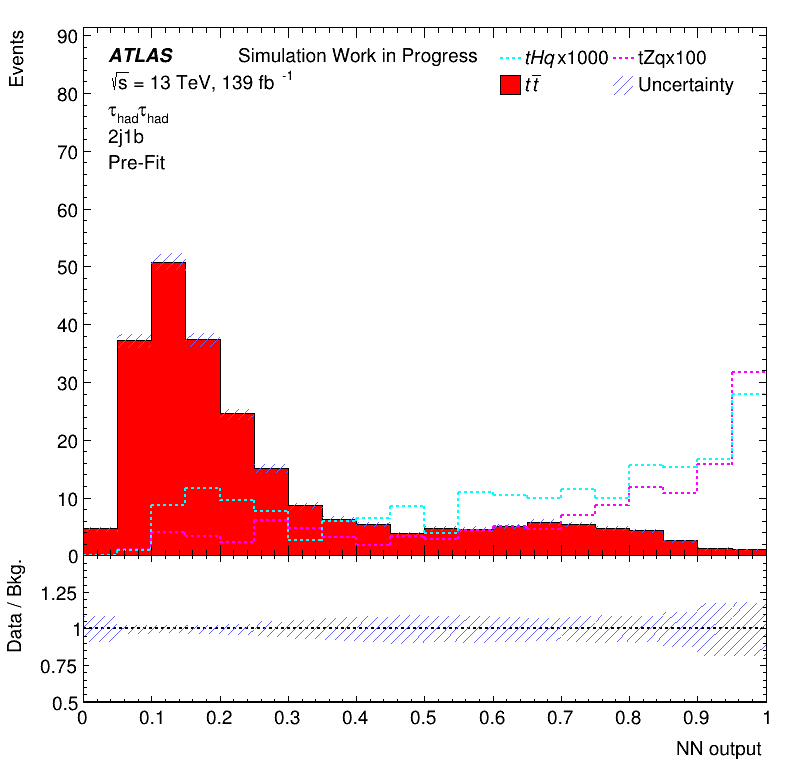
\includegraphics[width=\textwidth]{sgBkgComp}
            \end{figure}
        \end{column}
        \begin{column}{0.5\textwidth}
            \begin{itemize}
                \item Generally expected shape for signal and background response
                \item Due to the dominating size of \ttbar it defines the training
                \item For example \tZq gets classified as signal
                \item The network has to be trained to take care of smaller signal-like samples
                \item Approaches: multiple networks, multiple targets, reweighting of the samples
            \end{itemize}
        \end{column}
    \end{columns}
\end{frame}